% Standard Article Definition
\documentclass[]{article}

% Page Formatting
\usepackage[margin=1in]{geometry}
\setlength\parindent{0pt}

% Graphics
\usepackage{graphicx}

% Math Packages
\usepackage{physics}
\usepackage{amsmath, amsfonts, amssymb, amsthm}
\usepackage{mathtools}

% Extra Packages
\usepackage{pdfpages}
\usepackage{hyperref}
% \usepackage{listings}

% Section Heading Settings
% \usepackage{enumitem}
% \renewcommand{\theenumi}{\alph{enumi}}
\renewcommand*{\thesection}{Problem \arabic{section}}
\renewcommand*{\thesubsection}{\arabic{section}\alph{subsection})}
\renewcommand*{\thesubsubsection}{}%\quad \quad \roman{subsubsection})}

\newcommand{\Problem}{\subsubsection*{\textbf{PROBLEM:}}}
\newcommand{\Solution}{\subsubsection*{\textbf{SOLUTION:}}}
\newcommand{\Preliminaries}{\subsubsection*{\textbf{PRELIMINARIES:}}}

%Custom Commands
\newcommand{\N}{\mathbb{N}}
% \newcommand{\Z}{\mathbb{Z}}
% \newcommand{\Q}{\mathbb{Q}}
\newcommand{\R}{\mathbb{R}}
\newcommand{\C}{\mathbb{C}}

% \newcommand{\SigAlg}{\mathcal{S}}

% \newcommand{\Rel}{\mathcal{R}}

% \newcommand{\toI}{\xrightarrow{\textsf{\tiny I}}}
% \newcommand{\toS}{\xrightarrow{\textsf{\tiny S}}}
% \newcommand{\toB}{\xrightarrow{\textsf{\tiny B}}}

% \newcommand{\divisible}{ \ \vdots \ }
\newcommand{\st}{\ : \ }

% Theorem Definition
\newtheorem{definition}{Definition}
\newtheorem{assumption}{Assumption}
\newtheorem{theorem}{Theorem}
\newtheorem{lemma}{Lemma}
\newtheorem{proposition}{Proposition}
\newtheorem{remark}{Remark}
% \newtheorem{example}{Example}
% \newtheorem{counterExample}{Counter Example}


%opening
\title{
    MECH 6326 - Optimal Control and Dynamic Programming \\ 
    Homework 2
}
\author{Jonas Wagner\\ jonas.wagner@utdallas.edu}
\date{2023, March 3\textsuperscript{rd}}

\begin{document}

\maketitle

\tableofcontents

\newpage
\textbf{Dynamic Programming in Finite Space Systems}
% Problem 1 ----------------------------------------------
\section{Counting the number of policies}
Consider a stochastic optimal control problem:
\[
    \min E\qty[\sum_{k=0}^{N-1} g_k(x_k,u_k,w_k) + g_T(x_N,w_N)]
\]
With state $x_k \in \mathcal{X} = \{1,\dots,n\}$, input $u_k \in \mathcal{U} = \{1,\dots,m\}$, and disturbance $w_k \in \mathcal{W}=\{1,\dots,p\}$.
For finite state problems, the number of possible open- and closed-loop problems is finite.
Determine the number for each policy type below in terms of the cardinalities of these sets.
\footnote{Hint: Argue that for finite sets $A$ and $B$, the number of functions from $A$ to $B$ is $\abs{B}^{\abs{A}}$.}

\subsection{}
\Problem
An open loop policy: 
$u = (u_0,\dots,u_{N-1})$
$u \st \{0,\dots,N-1\} \to \mathcal{U}$
How many open-loop policies are there?
\Solution
\[
    \abs{\mathcal{U}}^\abs{\{0,\dots, N-1\}} = m^N
\]

\subsection{}
\Problem
A closed-loop policy is a sequence of functions: 
$\pi = (\pi_0,\dots,\pi_{N-1})$, where $\pi_k \st \mathcal{X} \to \mathcal{U}$.
How many closed-loop policies are there?
\Solution
\[
    \abs{\mathcal{U}}^\qty(\abs{\mathcal{X}}^\abs{\{0,\dots,N-1\}}) = m^\qty(n^N)
\]

\subsection{}
\Problem
A closed-loop policy in which the disturbance is known ahead of time:
$\phi = (\phi_{0},\dots,\phi_{N-1})$, where $\phi_{k} \st \mathcal{X}\cross \mathcal{W} \to \mathcal{U}$.
(i.e.) $u_k = \phi_k(x_k,w_k)$
How many of these closed-loop policies exist?
\[
    \abs{\mathcal{U}}^\qty(\abs{\mathcal{X} \cross \mathcal{W}}^\abs{\{0,\dots,N-1\}})
    = \abs{\mathcal{U}}^\qty(\qty(\abs{\mathcal{X}} \abs{\mathcal{W}})^\abs{\{0,\dots,N-1\}})
    = m^\qty((n\cdot p)^N)
\]


\newpage
% Problem 2 ----------------------------------------------
\section{A simple stochastic optimal control problem}
Consider the system\[
    x_{k+1} = w_{k}(x_k + u_k), \quad k = 0,1,2
\] with $u_k \in \{-1,0,1\}$, $w_k \in \{0,1\}$, and initial state $x_0 = -1$.
The disturbance $w_k$ is described by\[
    \begin{cases}
        P[w_k = 0] = 1 & \abs{x_k + u_k} > 1\\
        P[w_k = 0] = 0.5, P[w_k = 1] = 0.5 &\abs{x_k + u_k} \leq 1
    \end{cases}
\]
The cost function to be minimized is \[
    u_0^2 + u_1^2 + (x_1 + 1)^2 + (x_2 - 1)^2
\]

\subsection{}
\Problem
Determine the state space $\mathcal{X}_k$ for $k = 1,2$.
(i.e) based on $u_k$ and $w_k$, determine the possible values of $x_k$.
\Solution
Notation: $(x_k,u_k,w_k)$

For $k=0$, we have: $x_0 = -1$, $u_0\in \{-1,0,1\}$, and $w_0 \in \{0,1\}$.
\begin{multline}
    (x_0,u_0,w_0) \in \{
        (-1,-1,0), 
        % (-1,-1,1), Not reachable
        (-1,0,0),
        (-1,0,1),
        (-1,1,0),
        (-1,1,1)
    \}
\end{multline}

Thus, at $k=1$, with $x_1 = w_0 (x_0 + u_0)$, we have
\begin{multline}
    x_1 \in \{
        (-1,-1,0) \to x_1 = 0(-1-1) = 0, 
        % (-1,-1,1) \to x_1 = 1(-1-1) = 1, Not reachable
        (-1,0,0) \to x_1 = 0(-1+0) = 0,\\
        (-1,0,1) \to x_1 = 1(-1+0) = -1,
        (-1,1,0) \to x_1 = 0(-1+1) = 0,
        (-1,1,1) \to x_1 = 1(-1+1) = 0
    \} = \{-1,0\}
\end{multline}

Therefore, $x_1 \in \{-1,0\}$, $u_1 \in \{-1,0,1\}$, and $w_1 \in \{0,1\}$.
\begin{multline}
    (x_1,u_1,w_1) \in \{
        (-1,-1,0), 
        % (-1,-1,1), Not reachable
        (-1,0,0),
        (-1,0,1),
        (-1,1,0),
        (-1,1,1),\\
        (0,-1,0), 
        (0,-1,1),
        (0,0,0),
        (0,0,1),
        (0,1,0),
        (0,1,1)
    \}
\end{multline}

Thus, at $k=2$, with $x_2 = w_1(x_1 + u_0)$ we have

\begin{multline}
    x_2 \in \{
        (-1,-1,0) \to x_2 = 0(-1-1) = 0, 
        % (-1,-1,1) \to x_2 = 1(-1-1) = 1, Not reachable
        (-1,0,0) \to x_2 = 0(-1+0) = 0,\\
        (-1,0,1) \to x_2 = 1(-1+0) = -1,
        (-1,1,0) \to x_2 = 0(-1+1) = 0,
        (-1,1,1) \to x_2 = 1(-1+1) = 0,\\
        (0,-1,0) \to x_2 = 0(-1-1) = 0, 
        (0,-1,1) \to x_2 = 1(0-1) = -1,
        (0,0,0) \to x_2 = 0(0+0) = 0,\\
        (0,0,1) \to x_2 = 1(0+0) = 0,
        (0,1,0) \to x_2 = 0(0+1) = 0,
        (0,1,1) \to x_2 = 1(0+1) = 1
    \} = \{-1,0,1\}
\end{multline}

For the trajectory of $x_k$, we have $(x_0,x_1,x_2) \in \mathcal{X} \subseteq \mathcal{X}_0 \cross \mathcal{X}_1 \cross \mathcal{X}_2 = \{-1, 0, 1\}$.
$\mathcal{X}$ specifically though is actually more restrictive and is given as follows:\[
    \mathcal{X} = \{
        (-1, -1, -1),
        (-1, -1, 0),
        % (-1, 0, 1), Not reachable
        (-1, 0, -1),
        (-1, 0, 0),
        (-1, 0, 1)
    \}
\]

\subsection{}
\Problem
Compute the optimal cost-to-go functions $J_0(x)$ and $J_1(x)$ and optimal control policy $\pi = (\pi_0,\pi_1)$ using the dynamic Programming algorithm.
\Preliminaries
\begin{definition}
    \underline{\textbf{\emph{Optimal Control Policy:}}}
    The optimal control policy, $\pi^* = \{\mu_0^*, \dots, \mu_{N-1}^*\}, u_k^* = \mu_k^*(x_k)$, is defined where $\mu_k^*(x_k)$ minimizes the cost function \[
        J_k(x_k) = \min_{u_k \in \mathcal{U}_k} E_{w_k} \qty(g_k(x_k,u_k,w_k) + E[J_{k+1}(f_k(x_k,u_k,w_k))])
    \] that is propagated backwards in time from $N-1$ to $0$ where $J_N(x_N) = g_N(x_N)$.

    \textbf{Note:}
    When we are dealing with a finite state system, $x_k = i \in \mathcal{X}_k$ and $x_{k+1}=j = \mathcal{X}_{k+1}$, the problem can be simplified to minimize $J_k(x_k)$ as follows\[
        J_k(x_k=i) = \min_{u \in \mathcal{U_k(x_k=i)}} \qty(
            g(x_k=i, u) + \sum_{x_{k+1}=j} p_{ij}(u) J_{k+1}(x_{k+1})
        )
    \] where $p_{ij}(u) = P\qty(x_{k+1} = j \st x_k = i, u_k = u)$.
\end{definition}
\Solution
We take $N=2$ meaning that $J_N(x_N) = J_2(x_2) = (x_2 -1)^2$.
Thus, for each $x_2 \in \mathcal{X}_2$ we have: 
\[\begin{aligned}
    J_2(x_2 = -1) = (-1-1)^2 = 4\\
    J_2(x_2 = 0) = (0-1)^2 = 1\\
    J_2(x_2 = 1) = (1-1)^2 = 0
\end{aligned}\]

For $k=1$, \[
    J_1(x_1) = \min_{u_1 \in \mathcal{U}_1} E_{w_1} \qty[g_1(x_1,u_1,w_1) + J_{2}(f_1(x_1,u_1,w_1))]
\] and since $\mathcal{X}_k$ is finite, we can solve this simplistically for $x_1 \in \mathcal{X}_1$.

The probabilities for $k=1 \to k=2$ are given as follows:
Let $P(u_k) = \{p_{ij}(u_k)\}$, \[
    P(u_1 = -1) = \mqty[
        0 & 0.5\\
        1 & 0.5\\
        0 & 0
    ]
\]\[
    P(u_1 = 0) = \mqty[
        0.5 & 0\\
        0.5 & 1\\
        0 & 0
    ]
\]
\[
    P(u_1 = 0) = \mqty[
        0 & 0\\
        1 & 0\\
        0 & 0.5
    ]
\]

For $x_1 = -1$, we have $g_1(x_1,u_1) = u_1^2 + (x_1+1)^2$
\begin{multline}
    J_1(x_1=-1) = \min_{u_1 \in \{-1,0,1\}} \qty(
        (-1+1)^2 + u_1^2 + \sum_{j} p_{-1, j}(u_1) J_2(f(x_1)=j)
    ) \\
    = \min_{u_1 \in \{-1,0,1\}} u_1^2 + \sum_{j} p_{-1, j}(u_1) J_2(x_2=j)
    % = \min \mqty{
    %     u_1 = -1 \implies p_{-1,-1}(-1) J_2(-1) + p_{-1,0} J_2(0) + p_{-1,1} J_2(1) = (0)(4) + (1)(1) + (0)(0) = 1\\
    %     u_1 = 0 \implies p_{-1,-1}(0) J_2(-1) + p_{-1,0}() J_2(0) + p_{-1,1} J_2(1) = (0)(4) + (1)(1) + (0)(0) = 1\\
    % }
    \dots
\end{multline}
or equivalently,
\begin{multline}
    \mqty(J_1(-1)\\ J_1(0)) = \mqty((-1+1)^2\\(0+1)^2) +
        \min_{u} \mqty(u^2\\u^2) + P(u)^T \mqty[J_2(-1)\\J_2(0)\\J_2(1)] = \mqty(
        \min_{u} \mqty(u^2\\u^2) + P(u)^T \mqty[4\\1\\0]
    )\\
    = \mqty(0\\1) + \min \qty{
        u_1=-1 \implies \mqty(0\\1) + \mqty(1\\1) + \mqty[
        0 & 0.5\\
        1 & 0.5\\
        0 & 0
    ]^T \mqty[4\\1\\0],
    u_1 = 0 \implies \mqty(0\\1) + \mqty(0\\0) +  \mqty[
        0.5 & 0\\
        0.5 & 1\\
        0 & 0
    ]^T \mqty[4\\1\\0],
    u_1 = 1 \implies \mqty(0\\1) + \mqty(1\\1) +  \mqty[
        0 & 0\\
        1 & 0.5\\
        0 & 0.5
    ]^T\mqty[4\\1\\0]
    } \\
    = \min \qty{
        \mqty[2\\4.5],
        \mqty[2.5\\2],
        \mqty[2\\2.5]
    }
\end{multline}
We have \[
    \mqty(J_1(-1)\\ J_1(0)) = \mqty(2\\2)
\] with $\mu(-1) = 1$ and $\mu(0) = 0$

For $k=0$ the process is simpler:\[
    P_0(-1) = \mqty[0\\1]
\]\[
    P_0(0) = \mqty[0.5\\0.5]
\]\[
    P_0(1) = \mqty[0\\1]
\]

Then we have \begin{multline}
    J_0 = \min_{u} u_0^2 + P(u_0)^T\mqty[J_1(-1)\\J_1(0)]
    = \min \qty{
        (-1)^2 + \mqty[0&1] \mqty(2\\2.5),
        (0)^2 + \mqty[0.5&0..5] \mqty(2\\2.5),
        (1)^2 + \mqty[0&1] \mqty(2\\2.5),
    }\\
    = \min \qty{
        (-1)^2 + \mqty[0&1] \mqty(2\\2.5),
        (0)^2 + \mqty[0.5&0..5] \mqty(2\\2.5),
        (1)^2 + \mqty[0&1] \mqty(2\\2.5)
    } \\
    = min \qty{
        1+2.5,
        0+ 2.25,
        1+2.5
    }
    = min \qty{
        3.5,
        2.25,
        3.5
    }
    = 2.25
\end{multline}
Thus $u_0 = 0$.

The optimal control policy becomes:
    $\pi = (\pi_0, \pi_0)$
    with $\pi_0 = 0$ and \[ 
        p_1 = \begin{cases}
            0 & x_1 = -1\\
            1 & x_1 = 0
        \end{cases}
\]

% Problem 3
\newpage
\section{Another simple stochastic optimal control problem}
Consider a system with state $x \in \mathcal{X} = \{1,2\}$, input $u \in \mathcal{U} = \{1,2\}$, disturbance $w \in \mathcal{W} = \{1,2\}$, update equation \[x_{k+1} = f_k(x,u,w) = u\], and cost function \[
    g_k(x,u,w) = \begin{cases}
        -1 & x = u = 1, w=1,\\
        (k-1)^2 & x=1, u=2\\
        0 &\text{otherwise}
    \end{cases}
    \quad g_{N} = \begin{cases}
        0 & x=2\\
        \infty & \text{otherwise}
    \end{cases}
\]
Suppose $x_0 = 1$, $N = 4$, and $w_k$ are i.i.d. random variables with \[
    P(w_k = 1) = 0.3, \quad P(w_k=2) = 0.7
\]

\subsection{}
\Problem
Based on your results from Problem 1, how many open-loop, closed-loop state feedback, and closed-loop disturbance state feedback policies are there? 
This gives are rough idea of how many computations would need to be performed to compute the optimal policy by brute force.
\Solution
\subsubsection{Open-loop}
\[
    \abs{\mathcal{U}}^\abs{\{0,\dots, N-1\}} = m^N = (2)^(4) = 16
\]
\subsubsection{Closed-loop state feedback}
\[
    \abs{\mathcal{U}}^\qty(\abs{\mathcal{X}}^\abs{\{0,\dots,N-1\}}) = m^\qty(n^N) = (2)^\qty(2^4) = 2^16 = 65536
\]
\subsubsection{Closed-loop state and disturbance feedback}
\[
    \abs{\mathcal{U}}^\qty(\abs{\mathcal{X} \cross \mathcal{W}}^\abs{\{0,\dots,N-1\}})
    = \abs{\mathcal{U}}^\qty(\qty(\abs{\mathcal{X}} \abs{\mathcal{W}})^\abs{\{0,\dots,N-1\}})
    = m^\qty((n\cdot p)^N)
    = 2^\qty((2 \cdot 2)^4)
    = 2^(4^4)
    = 2^256
    \approx 1.15 \cdot 10^77
\]

\subsection{}
\Problem
Compute the optimal policy and value functions using the dynamic programming algorithm for (i) state feedback and (ii) state and disturbance feedback.

\Solution
\subsubsection{State Feedback}
Since the cost function is only ever dependent on the current state, input, and disturbance it forward/backward propagation over multiple timesteps is unnecessary.

For determining $u_3$, everything is unimportant outside of knowing $g_4$ is infinity unless $u_3 = 2$; thus, $\pi_3(\cdot) = 2$.

For $k=3$, we determined that $u_3 = \mu_3^* = 2$ \[
    J_3 = \begin{cases}
        (3+1)^2 + 0=16& x_3=1, u_3 = 2\\
        0 &x_3 \neq 1, u_3 = 2\\
        \infty & u_3 \neq 2
    \end{cases}
\]

For $k=2$,\[
    g_2 = \begin{cases}
        (0.3)(-10) + (0.7)(0) + 16 = 13 &x_2=1, u_2 = 1\\
        (2+1)^2 + 0 = 9 &x_2 = 1, u_2 = 2\\
        0 + 16 = 16 &x_2\neq 1, u_2 = 1\\
        0 + 0 &x_2 \neq 1, u_2 = 2
    \end{cases}
\] thus we have $\pi_2(\cdot) = 2$ with \[
    J_2(x_2 = 1) = 9, \quad J_2(x_2 = 2) = 0
\]

For $k=1$, \[
    g_1 = \begin{cases}
        (0.3)(-10) + (0.7)(0) + 9 = 6 &x_1=1, u_1 = 1\\
        (1+1)^2 + 0 = 4 &x_1 = 1, u_1 = 2\\
        0 + 9 = 9 &x_1 = 2, u_2 = 1\\
        0 + 0 &x_2 =2, u_2 = 2
    \end{cases}
\] thus we have $pi_1(\cdot) = 2$ with \[
    J_1(x_1 = 1) = 4, \quad J_2(x_1 = 2) = 0
\]

For $k=0$, \[
    g_1 = \begin{cases}
        (0.3)(-10) + (0.7)(0) + 4 = 1 &x_0=1, u_0 = 1\\
        (0+1)^2 + 0 = 1 &x_0 = 1, u_0 = 2
    \end{cases}
\] thus we have $pi_0(\cdot) = 1$  (or 2) with \[
    J_0 = 1
\]

\subsubsection{State and Disturbance Feedback}
or determining $u_3$, everything is unimportant outside of knowing $g_4$ is infinity unless $u_3 = 2$; thus, $\pi_3(\cdot) = 2$.

For $k=3$, we determined that $u_3 = \mu_3^* = 2$ \[
    J_3 = \begin{cases}
        (3+1)^2 + 0=16& x_3=1, u_3 = 2\\
        0 &x_3 \neq 1, u_3 = 2\\
        \infty & u_3 \neq 2
    \end{cases}
\]

For $k=2$,\[
    g_2 + g_3 = \begin{cases}
        -10 + 16 = 6 &x_2=1, u_2 = 1, w_2 = 1\\
        0 + 16 = 16 &x_2=1, u_2 = 1, w_2 = 2\\
        (2+1)^2 + 0 = 9 &x_2 = 1, u_2 = 2\\
        0 + 16 = 16 &x_2= 2, u_2 = 1\\
        0 + 0 &x_2 = 2, u_2 = 2
    \end{cases}
\] thus we have $\pi_2(\cdot) = 2$ with \[
    J_2(x_2 = 1) = 6, \quad J_2(x_2 = 2) = 0
\]

For $k=1$, \[
    g_1 + g_2= \begin{cases}
        -10 + 9 = -1 &x_1=1, u_1 = 1, w_1 = 1\\
        0 + 9 = 6 &x_1=1, u_1 = 1, w_1 = 2\\
        (1+1)^2 + 0 = 4 &x_1 = 1, u_1 = 2\\
        0 + 9 = 9 &x_1 = 2, u_2 = 1\\
        0 + 0 &x_2 =2, u_2 = 2
    \end{cases}
\] thus we have $pi_1(x_1=1,w_1=1) = 1$ otherwise $\pi_1 = 2$ with \[
    J_1(x_1 = 1, w_1 = 1) = -1, \quad J_1(x_1, w_1=2) = 6, \quad J_2(x_1 = 2) = 0
\]

For $k=0$, \[
    g_0 + g_1 = \begin{cases}
        -10 + -1 = -11 &x_0=1, u_0 = 1, w_0 = 1, w_1 = 1\\
        0 + -1 = -1 &x_0=1, u_0 = 1, w_0 = 2, w_1 = 1\\
        -10 + 6 = -4 &x_0=1, u_0 = 1, w_0 = 1, w_1 = 2\\
        0 + 6 = 6 &x_0=1, u_0 = 1, w_0 = 2, w_1 = 2\\
        (0+1)^2 -1 = 0 &x_0=1, u_0 = 2, w_1 = 1\\
        (0+1)^2 + 6 = 7 &x_0=1, u_0 = 2, w_1 = 2
    \end{cases}
\] thus we have $pi_0(\cdot) = 1$.


\newpage
\textbf{Markov Chains}
% Problem 4 ----------------------------------------------
\section{Markov Chain Distributions}
Consider a Markov Chain with the transition graph in \figurename \ \ref{fig:pblm4_markovchain}.

\begin{figure}[h]
    \centering
    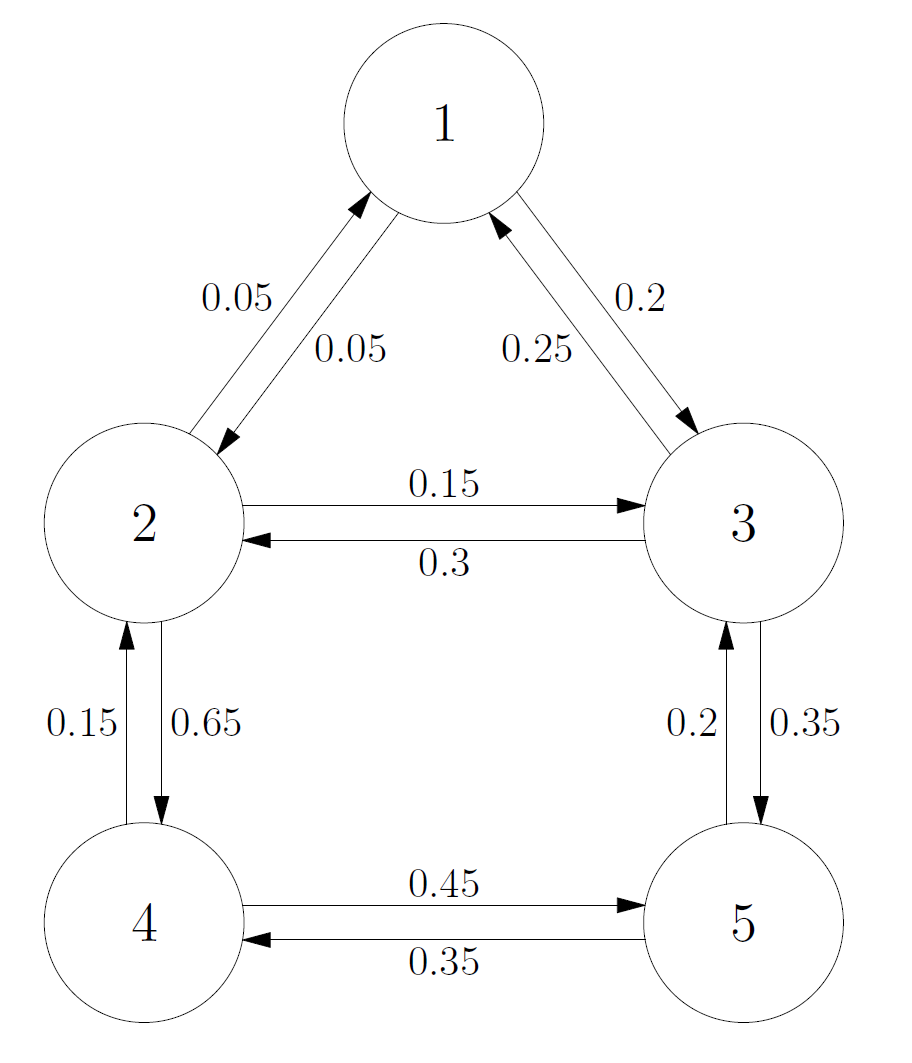
\includegraphics[width=0.25\textwidth]{figs/pblm4_markovchain.png}
    \caption{Markov Chain transition graph for Problem 4 (self-loops are omitted)}
    \label{fig:pblm4_markovchain}
\end{figure}

Suppose the initial state is $x_0 = 1$, and therefore $p_0 = \mqty[1&0&0&0&0]$.

\subsection{}
\Problem
Use distribution propagation to compute the following quantities at $N = 50$:
\begin{itemize}
    \item $P(x_N = 1)$
    \item $\frac{1}{N+1} \sum_{k=0}^N P(x_k = 1)$
\end{itemize}

\Solution
The Markov Chain in \figurename \ \ref{fig:pblm4_markovchain} is associated with the transition matrix \[
    P = \mqty[
        0.75    &0.05   &0.25   &0      &0\\
        0.05    &0.15   &0.3    &0.15   &0\\
        0.2     &0.15   &0.1    &0      &0.2\\
        0       &0.65   &0      &0.4    &0.35\\
        0       &0      &0.35   &0.45   &0.45
    ]
\]

Since the propagation of probabilities is given as \[
    p_{k+1} = p_{k} P
\] we have \[
    p_{k} = p_0 P^{k}
\] thus \[
    p_{N} = p_0 P^{N} 
\] which we can calculate with matlab.

The resulted probability for $P(x_N = 1)$ is the first element in $p_{N}$.

Similarly, the sum is the first element from the sum calculated as \[
    \frac{1}{N+1} \sum_{k=1}^N p_k
    = \frac{1}{N+1} \sum_{k=1}^N p_0 P^{k}
    = \frac{1}{N+1} p_0 \sum_{k=1}^N P^{k}
\] which can also be calculated in matalab.

\subsection{}
\Problem
Then use Monte Carlo estimation to approximate these quantities.
Generate plots of your estimates versus the number of sample trajectories used from 10 up to 10000 sample trajectories.
Compare the simulation results with the exact values computed previously.
\Solution

See attached MATLAB results.

Since there were issues publishing results, the plots are shown in \figurename \ \ref{fig:pblm4_fig1} and \figurename \ \ref{fig:pblm4_fig2}.

\begin{figure}[h]
    \centering
    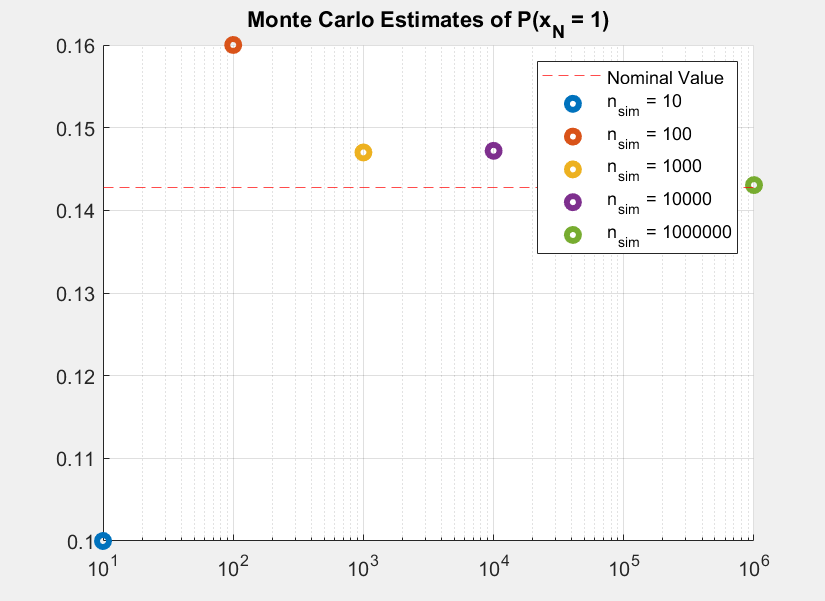
\includegraphics[width = 0.5\textwidth]{figs/pblm4_fig1.png}
    \caption{Monte Carlo Final Probability Estimate}
    \label{fig:pblm4_fig1}
\end{figure}

\begin{figure}[h]
    \centering
    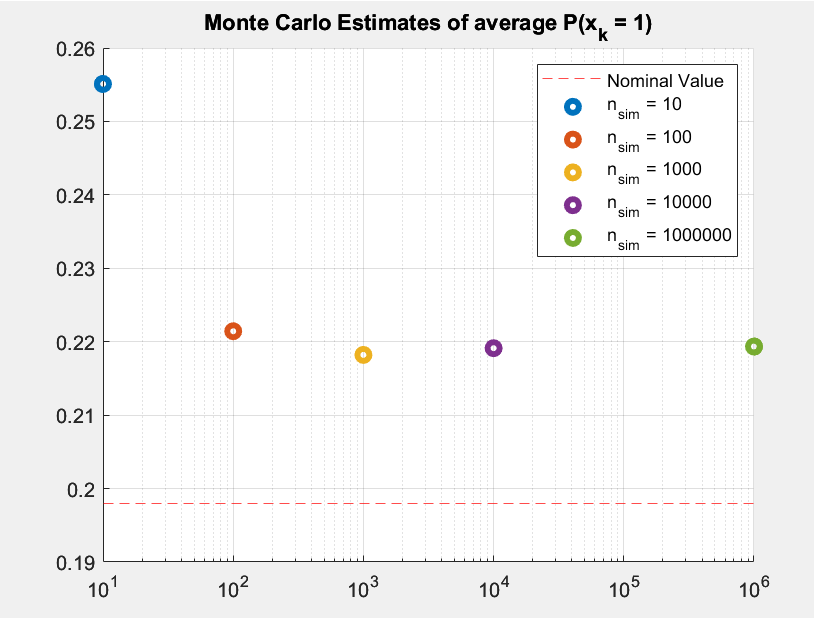
\includegraphics[width = 0.5\textwidth]{figs/pblm4_fig2.png}
    \caption{Monte Carlo Average Probability Estimate}
    \label{fig:pblm4_fig2}
\end{figure}

\newpage
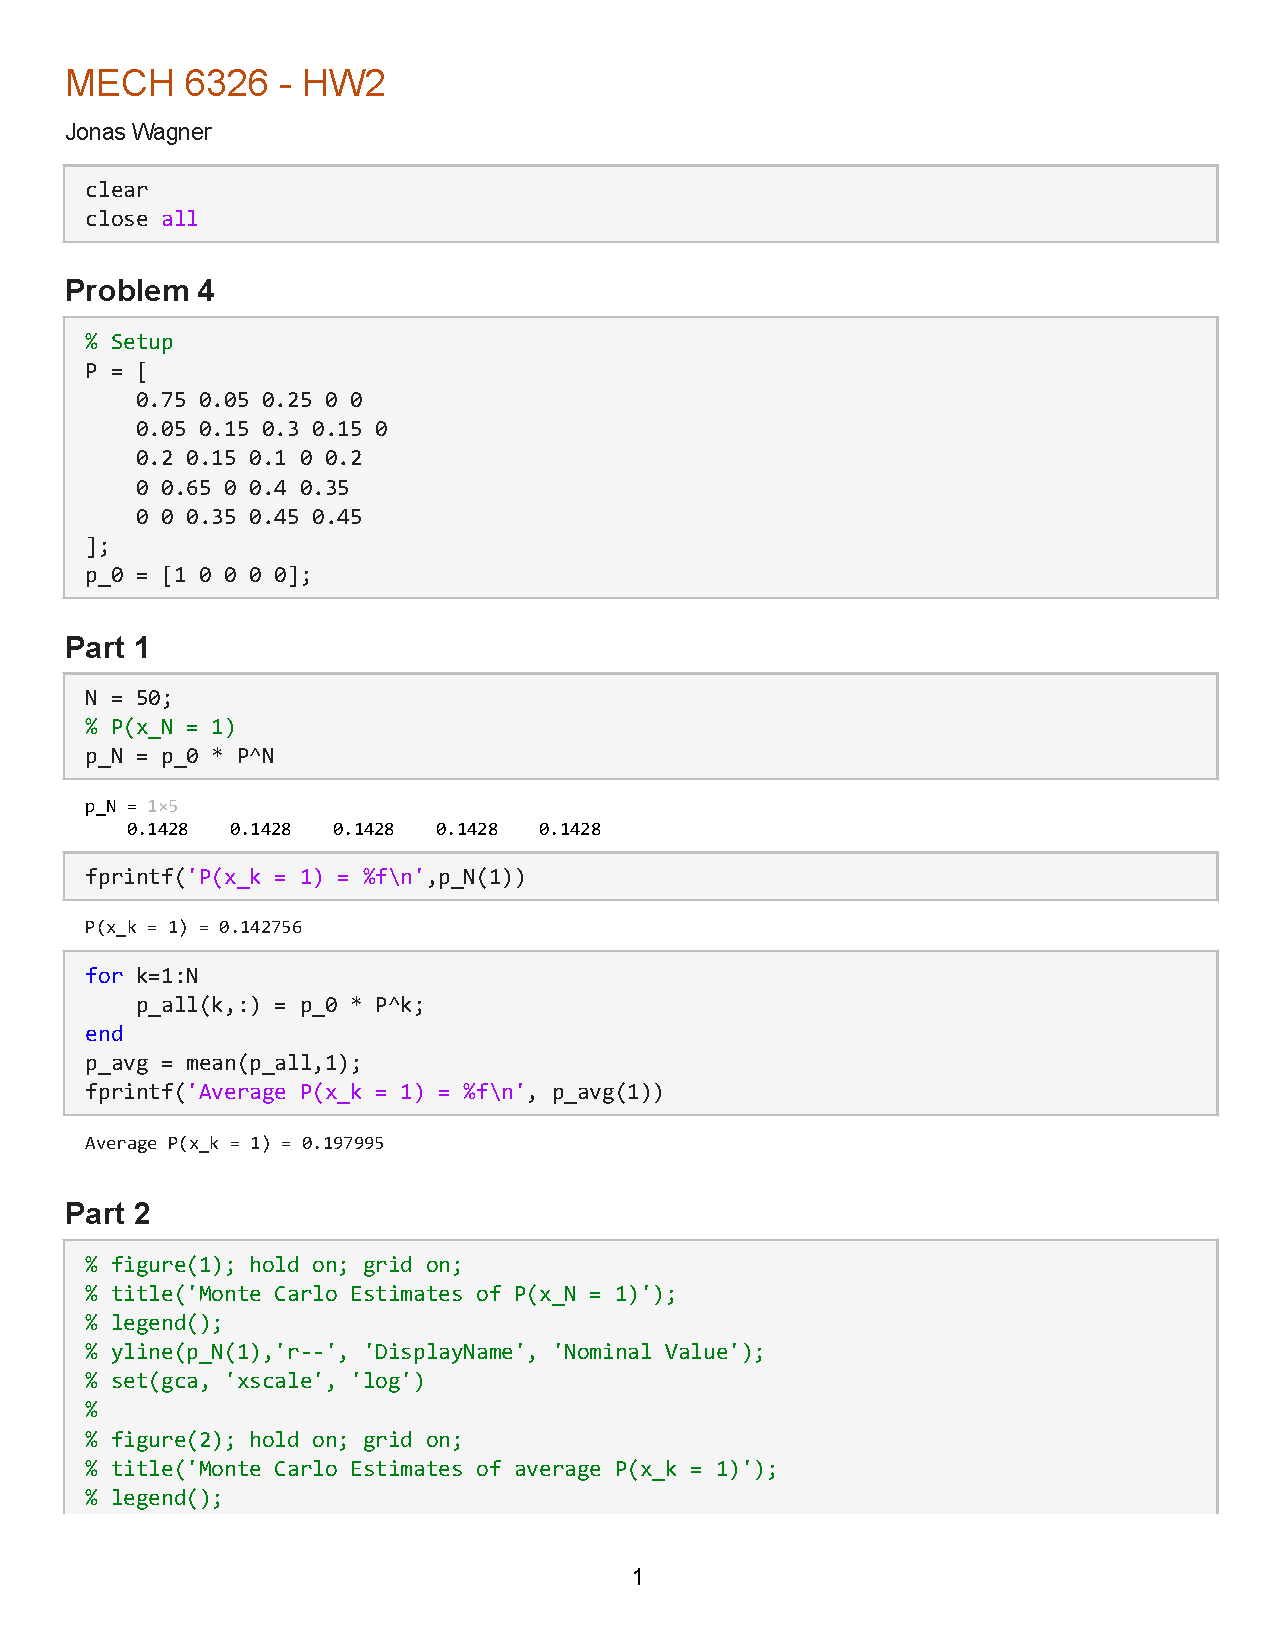
\includepdf[pages=-]{MECH6326_HW2.pdf}

% % Appendix ----------------------------------------------
% \newpage
% \appendix
% \bibliographystyle{plain}
% \bibliography{refs.bib}




\end{document}

